\chapter{Theory}\label{cha:theory}
\section{Rigid Body Dynamics}
According to~\cite{baberrigid} there are three major methods for solving rigid body
dynamics; penalty methods, impulse methods and constraint based methods.
In common with the methods for rigid body dynamics is the need for the governing laws of
motion which move the simulation forward in time, some form of collision detection
and a collision response. The collision detection, due to its planned use for GPU collision
detection, will be limited to a uniform grid/sort-based method, as described by~\cite{gpugems}.
The method of using mass splitting and spherical decomposition are very similar
to what~\cite{flex} and~\cite{bulletPipeline} have presented with regards to
constraint based physics, in this thesis I describe a method for using it with
impulse based physics while keeping the calculations on the GPU. When describing the laws of motion and equations
for updating the state variables the following diagram can be referenced.

\begin{figure}[H]
  \centering
  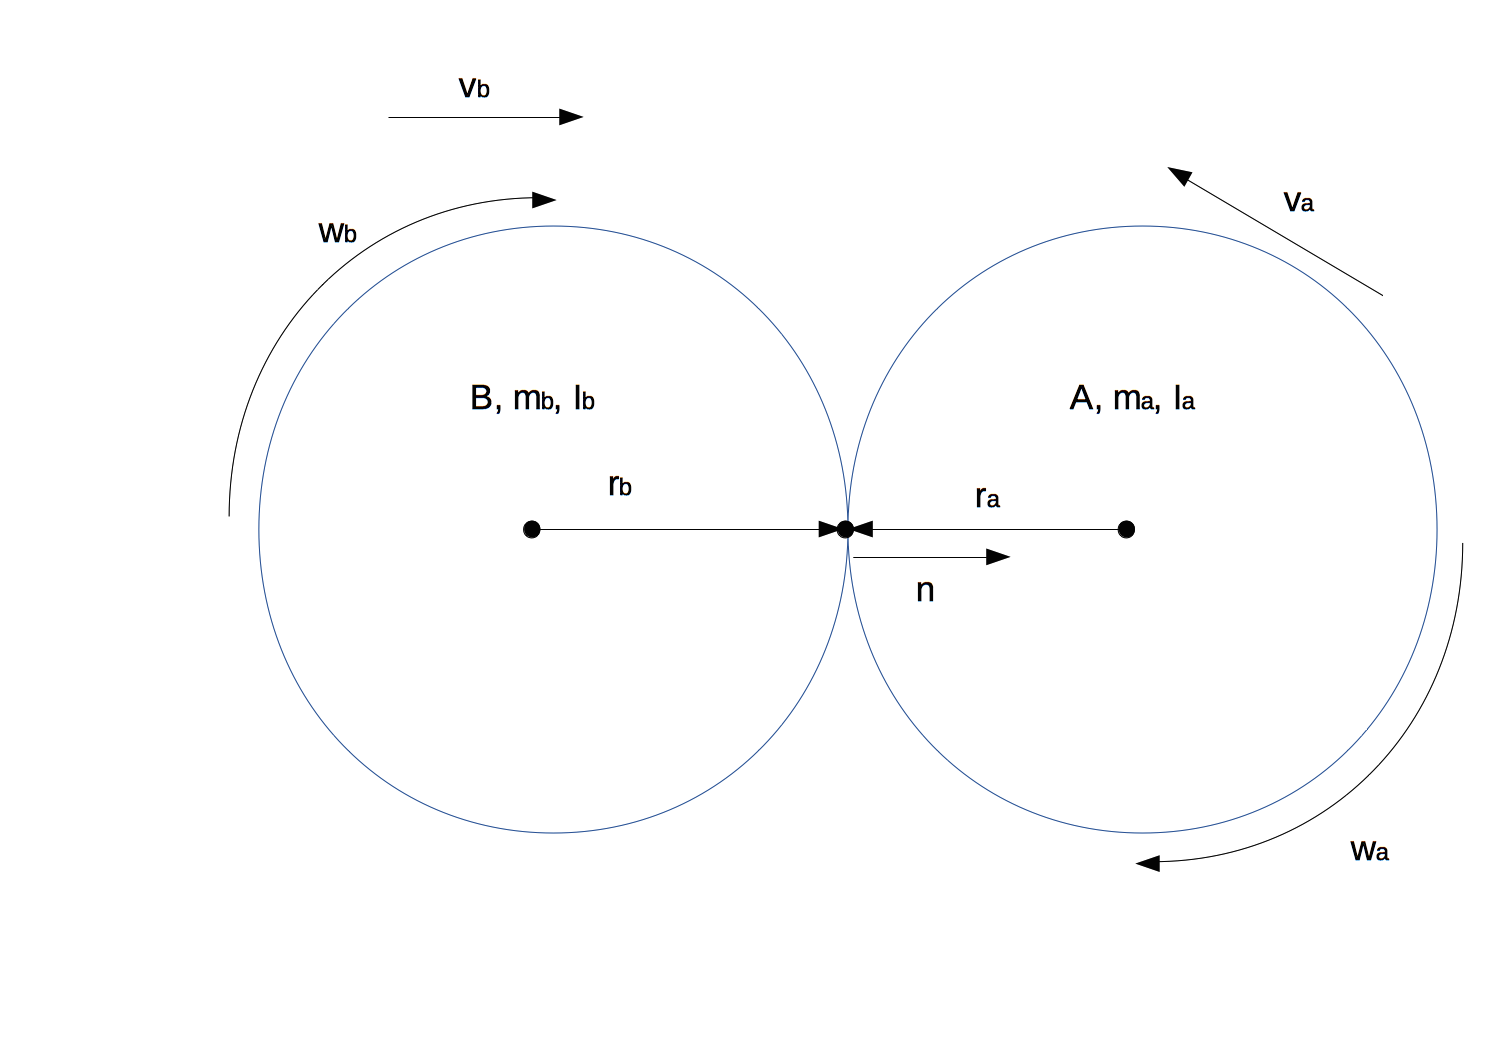
\includegraphics[width = 0.8\textwidth]{physicsscheme.png}
  \caption{Diagram of the relevant vectors and variables used when resolving a collision.}
  \label{fig:diag}
\end{figure}

\subsection{Laws of motion}
The following equations govern the motions of rigid bodies, these are quite
nicely summarized by~\cite{hansson}. They are repeated here for reference.

\begin{equation}
  \frac{d\vec{P}}{dt}=m\frac{d\vec{v}}{dt} = \vec{f}
\end{equation}

\begin{equation}
  \frac{d\vec{L}}{dt}=\vec{I}\frac{d\vec{\omega}}{dt} = \vec{\tau}
\end{equation}

\begin{equation}
  \frac{d\vec{x}}{dt}=\vec{v}
\end{equation}

\begin{equation}
  \frac{d\vec{q}}{dt} = \frac{1}{2}\vec{\omega}\vec{q}
\end{equation}

\begin{equation}
  \vec{I} = \vec{R}\vec{I}_0\vec{R}^T
\end{equation}

\subsection{Integrating the laws of motion discretely}
To use the equations in the previous subsection we need to be able to use them
discretely, for this purpose we need a discrete integration technique. The
simplest among them is the Euler step. With a fixed time step $\Delta t$, we
get the following equations that we can use to update the simulation one step
forward. The update for the quaternions are based on the description given by~\cite{fossum}.

\begin{equation}
  \vec{v}_{t + \Delta t} = \vec{v}_{t}+\frac{\vec{P}}{m}
\end{equation}
\begin{equation}
  \vec{L}_{t + \Delta t} = \vec{L}_{t}+\vec{\tau}\Delta t
\end{equation}

\begin{equation}
  \vec{\omega}_{t + \Delta t} = \vec{w}_t+\vec{I}^{-1}\vec{\tau}\Delta t
\end{equation}

\begin{equation}
  \vec{x}_{t + \Delta t} = \vec{x}_{t} + \vec{v}_t\Delta t
\end{equation}

\section{Spring-damper model}
Spring-damper model is the model for collision response described in~\cite{gpugems}.
The model has the benefit of being quite easy to implement on both CPU and GPU.
However, since there are two design parameters, the spring coefficient and the damping
constant, the system can be hard to tune. Often a parameter constellation that works
fine for one system will fail for another.
% Usually one need very small
% time steps as well since it does not handle interpenetration particularly gracefully.
% The system can give rise to mushy physics, hard spheres colliding with each other
% slow down, inter-penetrate, then accelerate outwards from each other.

The equations below describe how the force and torque can be derived for this type
of model. The equations describe the forces for collision between sphere i and j,
where k is the spring constant, c the damping constant and d the
diameter of the sphere. In equation~\ref{eq:tangent}, $\hat{r}$ refers to the
position of the particle relative to the body's center.

\begin{equation}
  \vec{f}_{i,spring} = -k(d-|\vec{r}_{ij}|)\frac{\vec{r}_{ij}}{|\vec{r}_{ij}|}
\end{equation}

\begin{equation}
  \vec{f}_{i,damping} = -c\vec{v}_{ij}
\end{equation}

\begin{equation}
  \vec{v}_{ij} = \vec{v}_{particle} + \vec{v}_{tangential}
\end{equation}

\begin{equation}\label{eq:tangent}
  \vec{v}_{tangential} = \vec{\omega} \cross ( \vec{r}- \vec{\omega}\bullet\frac{\vec{\omega}}{|\vec{\omega}^2|})
\end{equation}

Note that the equations above are mass independent which might be one of the
reasons for it's common use with the particle method.

This method has two unknown parameters, c and k, which must be tuned for the
specific system for stability. Often this parameter is decided through testing
and the tests need to be redone for new setups.

\section{Impulse method}\label{sec:imp}
To use the impulse method we need to solve the impulse j. ~\cite{baraff} explains the details
and derivations of the results below and I recommend the interested reader to peruse
his work.

Solving physics using the impulse method has the benefit of having few external tuning
parameters. In the suggested implementation tuning parameters could be, $\Delta t$,
$\mu$ and the bias factor.

The following equation can be used to calculate the impulse created in the
collision between body A and body B.
Please note that $\vec{j} = j\vec{\hat{n}}$ holds for all collisions, the direction
of $\vec{j}$ is always parallel to the collision normal by design.

\begin{equation}
  \vec{j} = \frac{-(1+\epsilon)\vec{v}_{rel,\vec{\hat{n}}}}
  {m_A^{-1}+m_B^{-1}+\vec{\hat{n}}\bullet(\vec{I}_A^{-1}(\vec{r}_A\cross\vec{\hat{n}})\cross\vec{r}_A
  +\vec{I}_B^{-1}(\vec{r}_B\cross\vec{\hat{n}})\cross\vec{r}_B)}
\end{equation}

The two following equations can be used to update the bodies' states.

\begin{equation}
  \Delta\vec{v}_A = \vec{j}m_A^{-1}
\end{equation}

\begin{equation}
  \Delta\vec{\omega}_A = \vec{j}\vec{I}_A^{-1}(\vec{r}_A\cross\hat{n})
\end{equation}

According to~\cite{hansson}, the same equations with a simple friction model can
be written as following.

\begin{equation}
  \Delta\vec{v}_A = \vec{j}m_A^{-1}(\vec{\hat{n}} - \mu\vec{\hat{t}})
\end{equation}

\begin{equation}
  \Delta\vec{\omega}_A = \vec{j}\vec{I}_A^{-1}(\vec{r}_A\cross(\vec{\hat{n}}-\mu\vec{\hat{t}}))
\end{equation}

With j redefined as the following.

\begin{equation}\label{eq:j}
  \vec{j} = \frac{-(1+\epsilon)\vec{v}_{rel,\vec{\hat{n}}}}
  {m_A^{-1}+m_B^{-1}+\vec{\hat{n}}\bullet(\vec{I}_A^{-1}(\vec{r}_A\cross(\vec{\hat{n}}-\mu\vec{\hat{t}}))\cross\vec{r}_A
  +\vec{I}_B^{-1}(\vec{r}_B\cross(\vec{\hat{n}}-\mu\vec{\hat{t}}))\cross\vec{r}_B)}
\end{equation}

In the equations the tangent can be calculated as described below.

\begin{equation}
  \vec{\hat{t}}=\frac{\vec{v}_{rel}-\vec{\hat{n}}(\vec{\hat{n}}\bullet\vec{v}_{rel})}{|\vec{v}_{rel}-\vec{\hat{n}}(\vec{\hat{n}}\bullet\vec{v}_{rel})|}
\end{equation}

\subsection{Replacing force with impulses}
Granted that we have the impulse created between body A and body B the following
equation can be used to update the states, the impulse is applied along the collision normal.
The equations regarding velocity updates are given below. In the equations below, $\vec{r}$,
is referring to the vector to the body's mass center. Please refer to figure~\ref{fig:diag}.

\begin{equation}
  \vec{\tau} = \vec{r}\cross\vec{f} = \vec{r}\cross\frac{\vec{j}}{\Delta t}
\end{equation}

\begin{equation}
  \vec{L}_{t+\Delta t} = \vec{L}_t + \vec\tau \Delta t = \vec{L}_t +(\vec{r}\cross\vec{f})\Delta t = \vec{L}_t + (\vec{r}\cross\vec{j})
\end{equation}

\begin{equation}
  \vec{\omega}_{t+\Delta t} = \vec{R}\vec{I}_0^{-1}\vec{R}^T\vec{L}_{t+\Delta t}
\end{equation}

\begin{equation}
  \vec{P}_{t+\Delta t} = \vec{P}_t + f\Delta t =\vec{P}_t+j
\end{equation}

\begin{equation}
  \vec{v}_{t+\Delta t} = \frac{\vec{P}_{t+\Delta t}}{m}
\end{equation}

The equations regarding position and orientation are given below.
\begin{equation}
  \vec{x}_{t+\Delta t} = \vec{x}_t+\vec{v}_{t+\Delta t}
\end{equation}

\begin{equation}
  \vec{a} = \frac{\vec{\omega}}{|\vec{\omega}|_2}
\end{equation}

\begin{equation}
  \theta = |\vec{\omega}\Delta t|_2
\end{equation}

\begin{equation}
  d\vec{q} = [\vec{a} sin(\frac{\theta}{2}),cos(\frac{\theta}{2})]
\end{equation}

\begin{equation}\label{eq:quat}
  \vec{q}_{t+\Delta t} = d\vec{q}*\vec{q}_t
\end{equation}

Note that the last multiplication in equation~\ref{eq:quat} is using a special quaternion multiplication, denoted with the asterisk.
With the quaternion defined as in equation~\ref{eq:quatDef}, the multiplication is performed as in equation~\ref{eq:quatMult}.

\begin{equation}\label{eq:quatDef}
  \vec{q} = [\vec{v},s] = [x\ y\ z\ s]
\end{equation}

\begin{equation}\label{eq:quatMult}
  \vec{q}_0*\vec{q}_1 = [s_0\vec{v}_1+s_1\vec{v}_0+\vec{v}_0\cross \vec{v}_1,s_0s_1-\vec{v}_0\bullet \vec{v}_1]
\end{equation}

The equations concerning quaternion updates closely follow what is described by~\cite{fossum}.
\subsection{Velocity biasing}
Since the equations laid out in the section above, assume a fixed time step there
arises situations where moving two spheres forward in time result in the spheres
interpenetrating. This situation has to either be resolved or somehow avoided.
To avoid this, one can calculate the first time of impact in the system globally and
resolve the collision at that point in time. This thesis will focus on how to resolve
the interpenetrations instead, due to time-backing not being particularly suitable
for parallel solvers or performance.
The method presented here is what is referred to as velocity biasing as described by~\cite{catto2006}.
When there is interpenetration we increase the relative velocity between the bodies
to ensure they separate properly. This is a penalty method, and solves a non-physical
phenomenon through a non-physical solution. Introducing large energies into the
system could potentially destabilize the system, therefore only a fraction of the
interpenetration is solved each iteration, and the impulse-velocity steps are iterated
several times instead to ensure smooth and careful solving of the interpenetration.
In addition a slop variable $\delta_{slop}$ is introduced so that some overlap of geometries
is allowed before correction starts. This relaxes the system on a whole somewhat.
Please refer to figure~\ref{fig:slop}.

\begin{figure}[H]
  \centering
  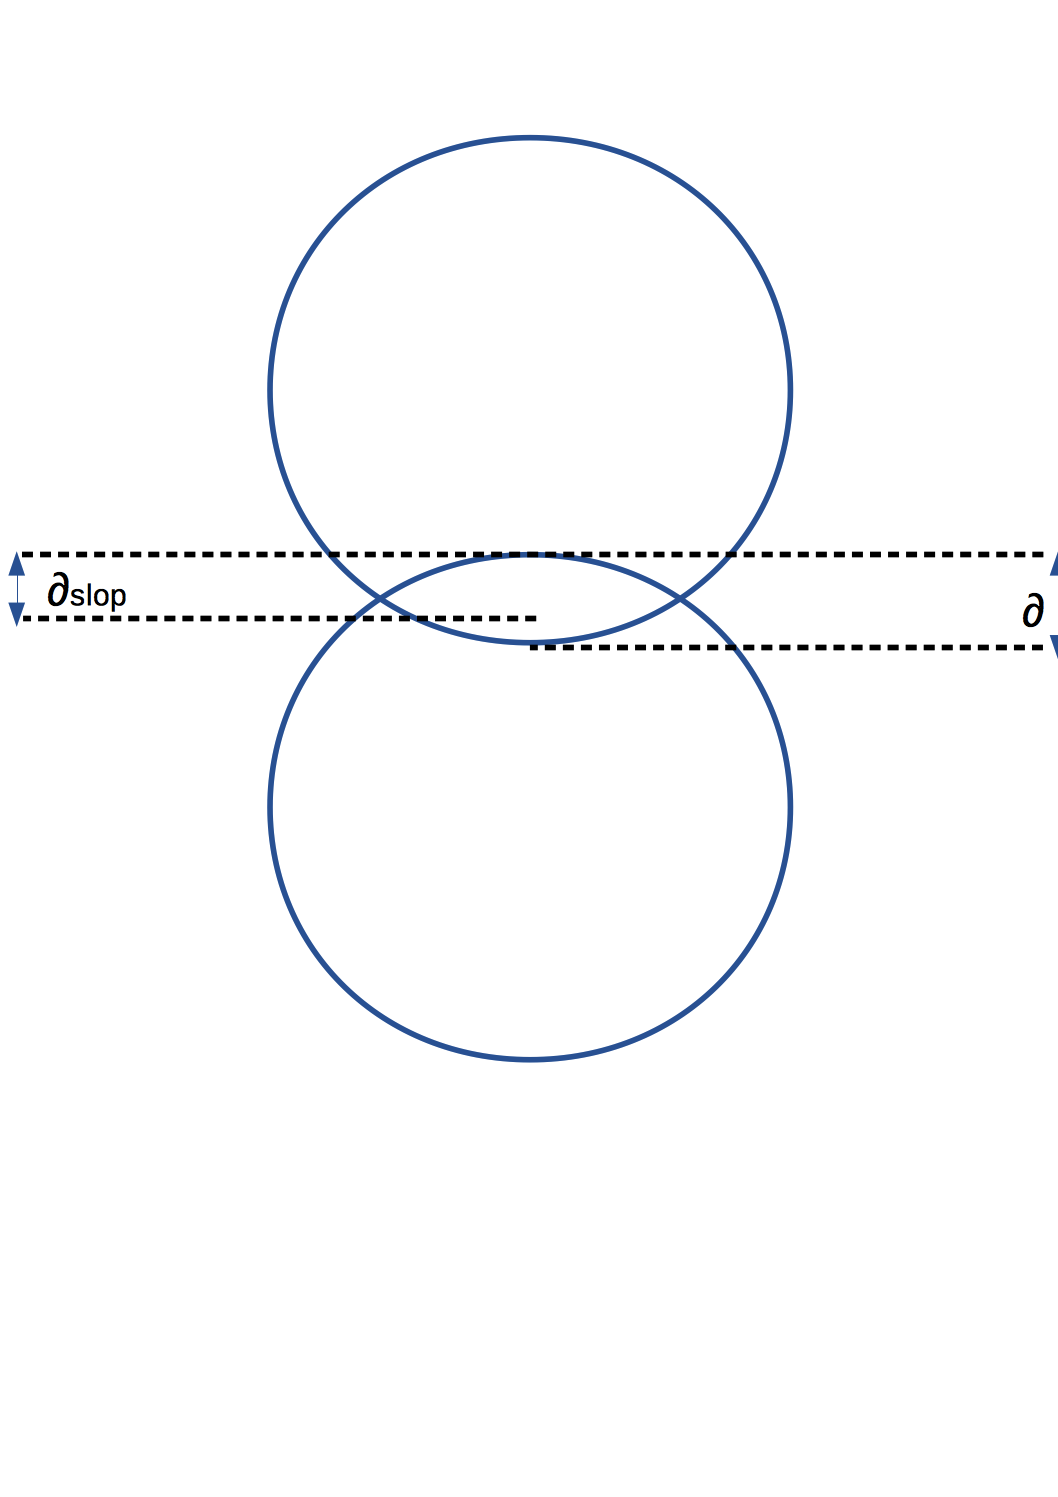
\includegraphics[width = 0.4\textwidth]{slop.png}
  \caption{Diagram of the relevant vectors and variables used when determining $\delta_{slop}$ and
  overlap. The figure is gathered from the presentation by~\cite{catto2006}.}
  \label{fig:slop}
\end{figure}

\begin{equation}
  v_{bias} = \frac{\beta}{\Delta t}max(0, \delta-\delta_{slop})
\end{equation}

Where $\beta$ between 0.1 and 0.3 are reasonable values according to~\cite{catto2006}.
With this, equation~\ref{eq:j} is modified to read the following.

\begin{equation}\label{eq:finalJ}
  \vec{j} = \frac{-(1+\epsilon)\vec{v}_{rel,\vec{\hat{n}}}-v_{bias}}
  {m_A^{-1}+m_B^{-1}+\vec{\hat{n}}\bullet(\vec{I}_A^{-1}(\vec{r}_A\cross(\vec{\hat{n}}-\mu\vec{\hat{t}}))\cross\vec{r}_A
  +\vec{I}_B^{-1}(\vec{r}_B\cross(\vec{\hat{n}}-\mu\vec{\hat{t}}))\cross\vec{r}_B)}
\end{equation}
% The impulse method can be used for both collision forces and contact forces
% according to~\cite{Lembcke}. There described as using Guendelman's time stepping
% algorithm. By, for example, detecting when the velocity is very small one can
% calculate the contact impulse by setting $\epsilon = 0$.
% Guendelman's time stepping algorithm is provided in pseudocode below, in accordance
% to what is described in~\cite{guendelman}.
%
% \begin{algorithm}[H]
%   \begin{algorithmic}[1]
%   \State DetectCollisions
%   \ForAll{collisions with v > 0}
%     \State calculateImpulses
%   \EndFor
%   \State applyGravity
%   \State updateVelocity
%     \ForAll{collisions with |v| <= $\epsilon_v$}
%       \State calculateImpulse (with elasticity = 0)
%     \EndFor
% \end{algorithmic}
% \end{algorithm}

\subsection{Inertia matrix}
To be able to simulate the rotations of the objects properly we need the objects
inherent property to resist rotation, the inertia tensor.
In 2D this is simply a single value, at least when considering rotation around
the center of mass. When moving to 3D we instead use a 3-by-3 matrix called the
inertia tensor. According to~\cite{ragnemalmscream} we can, when the objects initial
position is aligned with the objects principal axes, always write the inertia tensor
as a diagonal matrix.

By voxelizing the object which we seek the inertia tensor of and treating each voxel
as a point mass during the calculation we can sum over all the point masses and reach
an approximation of the inertia tensor. The method can be found described in
 'So How Can We Make Them Scream' by~\cite{ragnemalmscream}.
J can be calculated as following.

 \begin{equation}
  \vec{J} = \sum_i
  \begin{bmatrix}
    m_i(r_{iy}^2 + r_{iz}^2) & -m_ir_{ix}r_{iy} & -m_ir_{ix}r_{iz} \\
    -m_ir_{ix}r_{iy} & m_i(r_{ix}^2 + r_{iz}^2) & -m_ir_{iy}r_{iz} \\
    -m_ir_{ix}r_{iz} & -m_ir_{iy}r_{iz} & m_i(r_{ix}^2 + r_{iy}^2) \\
  \end{bmatrix}
 \end{equation}

 This method gets quite
 good results but is of course dependent on how finely one decomposes the object.
 Below is a comparison of theoretical versus approximated inertia tensor of a cube.
 Only one of the three diagonal components are presented since the object is symmetrical
 along all three axes the inertia tensor will have the same value along the diagonal.
 One can note that the inertia reaches a reasonable approximation quite quickly.


 \begin{figure}[H]
   \centering
   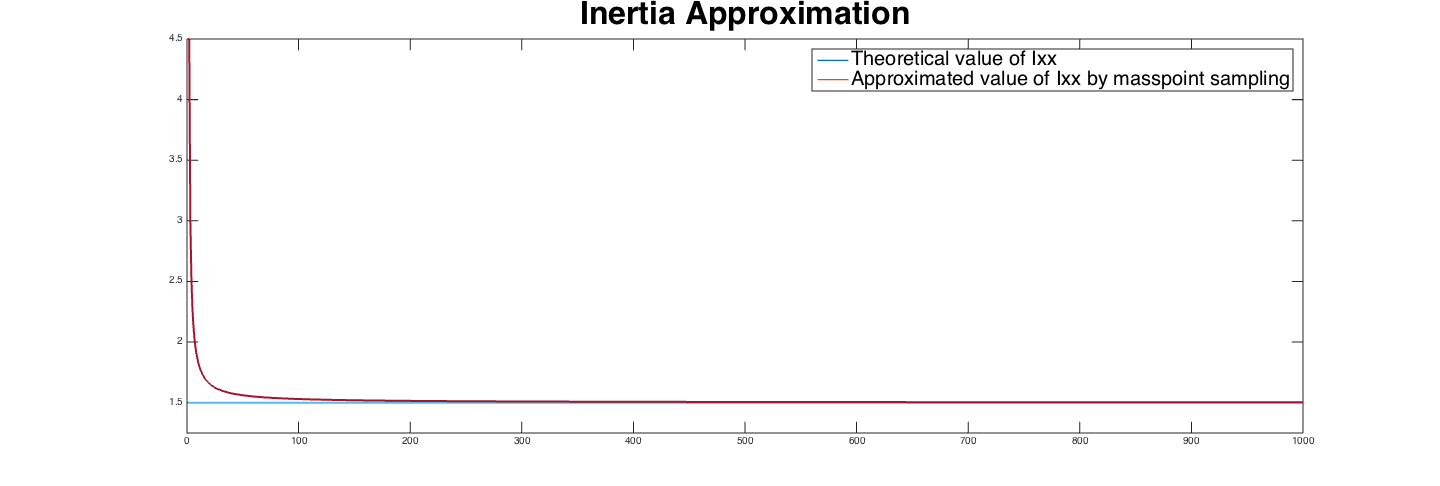
\includegraphics[width = \textwidth]{approximateIntertiaBoxSide3.png}
   \caption{Theoretical inertia versus approximated with increasing amounts of voxels.}
   \label{fig:appInertia}
 \end{figure}

% \section{Shock propagation}
% To be able to simulate a N-sphere long Newton cradle on can implement N-substep
% shock propagation. By impulse solving and updating the velocities but not the
% positions one can transfer the impulses N bodies away from the original impact.
% This works since all spheres in the cradle are in collision, but the negative
% (or zero) approach velocity stops the calculation of an impulse. However, if we
% calculate the original impulse and apply it to the velocity and reiterate a new
% collision becomes valid. The method can however only propagate the shock by the
% number of sub iterations allowed and the method can become somewhat expensive.
% Using narrowphase algorithms which are not predictive (as in projects the speed)
% and reusing the same collisions detected in each sub iteration saves a lot on
% performance. This whole algorithm is described, in short, in~\cite{lembcke}.
% Pseudocode for this is provided below. Notice that no new collisions are detected.
% \begin{algorithm}[H]
%   \begin{algorithmic}[1]
%     \State DetectCollisions
%     \While{iterations < subIterations}
%     \ForAll{collisions}
%     \State calculateImpulse
%     \EndFor
%     \State applyImpulses
%     \State updateVelocities
%     \EndWhile
%   \end{algorithmic}
% \end{algorithm}
%
% Maybe have this section?
% \section{Bullet Solver}
% \section{Bullet Broadphase}
% Bullet physics as most physics engines use a broadphase algorithm to narrow down
% the potential collisions which need to be handled by the solver. Early exclusion
% can reduce the problem from $O(N^2)$ to a reasonable $O(N)$.
% One of the methods that bullet provides is the so called Sweep-and-Prune (SAP),
% sometimes known as Sweep-and-Sort~\cite{gpugems}
% \subsection{Sweep and prune}
% Each object in the world is assigned an AABB (Axis-Aligned Bounding Box) and these
% boxes are then projected unto each of the axes X,Y,Z. A pair of boxes can have a
% potential collision if and only if the pair overlap on all axes
% (see separating axis theorem in for instance~\cite{ragnemalmpolygons}).
% The projection is a reduction in dimensionality which give a significant performance increase.
% In addition one can optimize the algorithm with some intelligent design decisions
% concerning array handling and keeping the arrays sorted. The details are quite nicely
% described by~\cite{SAPPierre} and is left up to the reader to peruse. \cite{bulletPipeline}
% talked about a parallel implementation of SAT during his talk at GDC.
